%COMANDO CHE DETERMINA IL TIPO DI DOCUMENTO CHE SI VUOLE CREARE

\documentclass[a4paper,12pt]{report}

%ELENCO DEI PACCHETTI UTILI PER LA STESURA DEL DOCUMENTO
\usepackage{enumitem}
\usepackage[utf8]{inputenc}
\usepackage[english, italian]{babel}
\usepackage{graphicx}
\usepackage{float}
\usepackage{tabularx}
\usepackage{makecell}
\usepackage{titlesec}
\usepackage{fancyhdr}
\usepackage{lastpage}
\usepackage{xurl}
\usepackage{hyperref}
\usepackage{geometry}
\usepackage[table,dvipsnames]{xcolor}
\setcounter{tocdepth}{5}
\setcounter{secnumdepth}{5}
\usepackage{caption}
\usepackage{etoolbox}% >= v2.1 2011-01-03
\usepackage{tikz}
\usepackage{listings}
\usepackage{scalerel}
\usepackage{longtable}
\captionsetup[table]{position=bottom}
\usepackage{comment}
\usepackage{listings}
%COMANDO PER AVERE IL CAPITOLO CON IL NOME CHE VOGLIAMO NOI

\titleformat{\chapter}
{\normalfont\bfseries\LARGE}{\thechapter}{20pt}{\LARGE}

%COMANDO PER LA SPAZIATURA DEI TITOLI DAL BORDO DEL FOGLIO

\titlespacing*{\chapter}{0cm}{0cm}{0.2cm}
\setlength{\headsep}{2cm} % spaziatura tra header e testo


%COMANDO PER LA SPAZIATURA DEL TESTO DAI BORDI LATERALI

\geometry{
	left=20mm,
	right=20mm,
}

%COMADNO PER AVERE L'INDICE DEL NOME CHE SI VUOLE

\renewcommand{\contentsname}{Indice}

%COMADNI PER OTTENERE SUBSUBSECTION NUMERATE E PRESENTI NELL'INDICE

\setcounter{tocdepth}{5}
\setcounter{secnumdepth}{5}

%COMANDI PER OTTENERE HEADER E FOOTER

\pagestyle{plain}

\fancypagestyle{plain}{
	\fancyhf{}
	\lhead{
\includegraphics[width=3cm]{./immagini/logo.png}}
	\chead{}
	\rhead{\fontsize{12}{10}Documento Tecnico}
	\lfoot{}
	\cfoot{\thepage\ di \pageref{LastPage}}
	\rfoot{}
}

\pagestyle{plain}

%COMANDI PER LINK

\hypersetup{
	colorlinks=true,
	linkcolor=black,
	filecolor=black,
	urlcolor=blue,
	citecolor=black,
}

%COMANDI PER SNIPPET DI CODICE

\BeforeBeginEnvironment{lstlisting}{\begin{mdframed}\vspace{-0.7em}}
	\AfterEndEnvironment{lstlisting}{\vspace{-0.5em}\end{mdframed}}

% needed for \lstcapt
\def\ifempty#1{\def\temparg{#1}\ifx\temparg\empty}

% make new caption command for listings
\usepackage{caption}
\newcommand{\lstcapt}[2][]{%
	\ifempty{#1}%
	\captionof{lstlisting}{#2}%
	\else%
	\captionof{lstlisting}[#1]{#2}%
	\fi%
	\vspace{0.75\baselineskip}%
}

\definecolor{atomlightorange}{rgb}{0.88,0.76,0.55}
\definecolor{atomdarkgrey}{RGB}{59,62,75}

% set listings
\lstset{%
	basicstyle=\footnotesize\ttfamily\color{atomlightorange},
	framesep=20pt,
	belowskip=10pt,
	aboveskip=10pt
}

% add frame environment
\usepackage[%
framemethod=tikz,
skipbelow=8pt,
skipabove=13pt
]{mdframed}
\mdfsetup{%
	leftmargin=0pt,
	rightmargin=0pt,
	backgroundcolor=atomdarkgrey,
	middlelinecolor=atomdarkgrey,
	roundcorner=6
}

%BIBLIOGRAFIA

\makeatletter
\def\thebibliography#1{\chapter*{Bibliografia\@mkboth
		{Bibliografia}{Bibliografia}}\list
	{[\arabic{enumi}]}{\settowidth\labelwidth{[#1]}\leftmargin\labelwidth
		\advance\leftmargin\labelsep
		\usecounter{enumi}}
	\def\newblock{\hskip .11em plus .33em minus .07em}
	\sloppy\clubpenalty4000\widowpenalty4000
	\sfcode`\.=1000\relax}
\makeatother

%DEFINIZIONE COLORI

\definecolor{airforceblue}{rgb}{0.36, 0.54, 0.66}
\hypersetup{
	colorlinks=true,
	linkcolor=black,
	filecolor=black,
	urlcolor=blue,
	citecolor=black,
}
\begin{document}
	\makeatletter
	\begin{titlepage}
		\begin{center}
			\vspace*{2,0cm}
			\author{Andrea Cecchin}
			\title{Documento Tecnico}
			\date{}
			
\includegraphics[width=0.5\linewidth]{./immagini/logo.png}\\[4ex]

			
			{\huge \bfseries  \@title }\\[2ex] 
			{\LARGE  \@author}\\[50ex]
			\vspace*{-9,0cm}
			
		\vspace{4cm}
		Il codice è disponibile nella repository pubblica di Github al seguente link:
		\begin{center}
			\url{https://github.com/NFT-Lab/back-end-spring}
		\end{center}
	\vspace{2cm}
		\hfill \break
		\fontsize{17}{10}\textbf{Sommario} \\
		\vspace{0.1cm}
		Il presente documento contiene le scelte architetturali che sono state implementate all'interno del progetto NFTLab. Contiene i design pattern e i diagrammi di attività, sequenza, classi e package.
		\end{center}
	\end{titlepage}
	\makeatother
	
	\tableofcontents{}

	\chapter{Architettura}
In questo capitolo viene descritta l'architettura del prodotto nelle sue componenti.
\section{Struttura generale del progetto}
\begin{center}
	\begin{figure}[H]
		\centering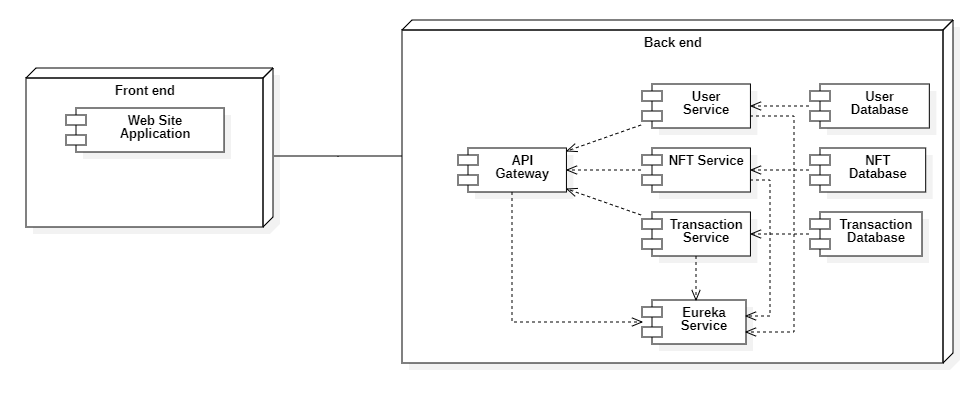
\includegraphics[scale=0.65]{./immagini/componentNFTLab.png}
		\caption{Diagramma UML dei componenti del back-end}
	\end{figure}
\end{center}
Il back-end sviluppato per il progetto è composto da cinque servizi, due di supporto (eureka e gateway) e tre per le funzionalità richieste. \\
L'API che svolge la funzionalità di gateway crea al suo avvio le route di collegamento ai servizi User, NFT e Transaction. Questo routing permette di attuare richieste HTTP rivolgendosi solamente al gateway senza essere a conoscenza dell'indirizzo privato di ogni servizio. Il gateway si prenderà cura di instradare correttamente le richieste verso ogni servizio rispondendo al client con i dati ricevuti. Il framework Spring permette la creazione di API gateway attraverso il pacchetto Spring Cloud Gateway, usando questa libreria infatti sarà solo necessario impostare le proprietà del file \emph{application.properties} e inserire la dipendenza nel file pom.xml per utilizzare tutte le sue funzionalità.

Una volta completati i due passaggi appena spiegati è necessario solo creare le route all'interno del controller dell'applicativo e l'autoconfigurazione di Spring si occuperà di generare le componenti autonomamente.
\\
Il servizio eureka invece è stato sviluppato usando il framework Spring Cloud Netflix che permette un'autoconfigurazione completa del servizio impostando solamente l'\emph{application.properties} e inserendo l'annotazione \emph{@EnableEurekaServer} nel file main del progetto Java.

I tre servizi che espongono le funzionalità del prodotto da sviluppare sono collegati a tre database diversi secondo l'architettura a microservizi. I database sono stati creati usando MySQL implementato dal programma XAMPP. 
\section{Struttura generale dei servizi}
Ogni servizio è composto dai tre livelli del pattern MVC: Presentation Layer, Business Logic Layer e Data Layer. Il Presentatio Layer viene definito nel package Controller, il controller definisce l'interfaccia con l'esterno e con la quale si può interagire con l'applicativo. Il Business Logic Layer viene definito nel package Service, in esso vengono manipolati i dati e formulate le risposte per ogni richiesta. Infine il Data Layer è definito attraverso il package Repository e il package dei modelli degli oggetti (User, Opera, Transaction etc), il repository è la classe che crea un collegamento al database attraverso i modelli degli oggetti creati utilizzando delle specifiche annotazioni, in questa classe possono essere definite query personalizzate oltre a quelle disponibili di default dal framework Spring Data JPA. Il package con al suo interno i modelli degli oggetti invece serve esclusivamente per la definizione delle entità.

	\chapter{Descrizione servizi}
In questo capitolo vengono descritti i servizi singolarmente in tutte le loro parti.
\section{Servizio Utenti}
Il servizio utenti (o User Service) è l'API che espone funzionalità per la registrazione, l'accesso e la modifica dei dati per l'utente. L'applicativo è composto dai seguenti package:
\begin{itemize}
	\item \textbf{Main}: contiene la classe main del progetto;
	\item \textbf{Controller}: contiene la classe Controller che definisce l'interfaccia dell'applicativo;
	\item \textbf{Service}: contiene la classe UserService che definisce i metodi per la modellazione delle richieste effettuate al controller lavorando con le entità;
	\item \textbf{Repository}: contiene l'interfaccia di connessione al database usando JpaRepository;
	\item \textbf{User}: contiene le classe che modella gli oggetti relativi all'utente.
\end{itemize}
\subsection{Controller}
Il controller del servizio utenti definisce sei metodi per l'utilizzo dei dati presenti nel database:
\begin{itemize}
	\item \textbf{Login}: metodo per l'accesso e restituzione dei dati dell'utente che vuole accedere;
	\item \textbf{SignUp}: metodo per la registrazione di un nuovo utente ed inserimento dello stesso nel database;
	\item \textbf{Change password}: metodo per il cambio della password, utilizza un oggetto particolare nella richiesta dei dati da inserire nel database;
	\item \textbf{Change data}: metodo per la modifica dei dati dell'utente nel database;
	\item \textbf{Get user by Id}: metodo interno per la restituzione dell'utente dato un determinato ID;
	\item \textbf{Get wallet by Id}: metodo per la restituzione dell'indirizzo del wallet dell'utente.
\end{itemize}
Gli ultimi due metodi vengono utilizzati internamente da servizio NFT e Transaction per ottenere le informazioni interne del database del servizio utenti.
I primi quattro metodi definiscono anche risposte in caso di errori nell'inserimento dei dati o controlli effettuati nella richiesta inviate dal client. Ogni risposta è definita utilizzando un HttpStatus diverso per ogni tipo di errore riscontrato.
\subsection{Service}
Il service è composto da metodi per l'inserimento, manipolazione e controllo dei dati, i più importanti sono:
\begin{itemize}
	\item \textbf{Add user}: metodo per l'inserimento di un nuovo utente nel database, questo metodo effettua anche l'hash della password;
	\item \textbf{Update User Password e Data}: due metodi per le corrispondenti modifiche ai dati dell'utente entrambi richiamano Add user per inserire le modifiche all'utente;
	\item \textbf{Check email e password}: metodo per il controllo dei due campi dell'utente per individuare la presenza dello stesso nel database.
\end{itemize}
Nel metodo per la modifica dei dati e della password viene utilizzato il metodo Add user perchè la logica per l'aggiornamento e inserimento dei dati è identica per entrambi i metodi grazie al metodo della JpaRepository \emph{.save()}.
\subsection{Repository}
Il repository contiene i metodi che utilizzano l'ORM per la creazione delle query personalizzate. Le query aggiuntive sono:
\begin{itemize}
	\item \textbf{Find Users by email}: query per la ricerca dell'utente in base alla email;
	\item \textbf{Exists user by email}: query per l'esistenza di un utente data l'email;
	\item \textbf{Exists user by email and password}: query per l'esistenza di un utente data l'email e la password.
\end{itemize}
\subsection{User}
Il package User contiene le classi degli oggetti che vengono utilizzati nell'applicativo. Gli oggetti sono:
\begin{itemize}
	\item \textbf{NFTUserRequest}: oggetto per le richieste da parte del servizio NFT;
	\item \textbf{User}: oggetto per la creazione di utenti e modellazione dei dati nel database;
	\item \textbf{UserPayload}: oggetto per la modifica della password.
\end{itemize}

\section{Servizio opere}
Il servizio opere (o NFT) è l'API che espone le funzionalità per l'inserimento, la modifica di opere nel database.
L'applicativo è composto dai seguenti package:
\begin{itemize}
	\item \textbf{Configuration}: package per la configurazione dei bean;
	\item \textbf{Controller}: contiene la classe dell'interfaccia dell'applicativo verso l'esterno;
	\item \textbf{File}: contiene la classe per la modellazione dei file e la scrittura su disco;
	\item \textbf{Main}: contiene la classe main;
	\item \textbf{Opera}: contiene le classi oggetti per la modellazione delle entità;
	\item \textbf{Repository}: contiene le interfacce per il collegamento al database;
	\item \textbf{Service}: contiene la classe per l'inserimento, modifica e controlli dei dati dalle richieste;
	\item \textbf{Transaction}: contiene la classe utilizzata per le richieste dal servizio transazioni;
	\item \textbf{User}: contiene la classe utilizzata per le richieste dal servizio utenti;
\end{itemize} 
\subsection{Configuration}
All'interno di questo package si trova il file di configurazione dei bean per la creazione del RestTemplate e dell'istanziazione del collegamento alla Blockchain. Quest'ultimo per essere configurato in una nuova macchina deve subire delle variazioni nel codice per effettuare il collegamento ad una blockchain locale. Viene utilizzato il programma Ganache per generare una blockchain locale con dei wallet fittizi caricati con un determinato numero di ether (ETH). Attraverso gli indirizzi messi a disposizione dal programma si modificherà la configurazione per creare d'apprima il contratto per la prima esecuzione del programma e poi si andrà ad effettuare il collegamento al contratto attraverso il metodo \emph{.loadContract()}.
Di seguito vengono descritti i passaggi per la creazione di un contratto:
\begin{enumerate}
	\item Si avvia un'istanza di Ganache per ottenere un portafoglio non vuoto;
	\item Si sceglie un indirizzo di un portafoglio a caso;
	\item Si sostituisce il metodo \emph{.loadContract()} con il metodo \emph{.deploy()};
	\item Inserisci i parametri necessari presi dalle variabili precedenti e nel nome e symbol inserisci due stringhe di riferimento per il progetto (es. "nft","nft-lab");
	\item Si effettua un ciclo di attivazione e spegnimento dell'applicativo per generare il contratto;
	\item Si modifica il metodo re-immettendo \emph{.loadContract()} con i parametri corretti;
	\item Avviando l'applicativo si caricherà il contratto e sarà disponibile finchè non si utilizzerà una nuova istanza di Ganache creata da zero.
\end{enumerate}
\subsection{Controller}
Il controller del servizio nft definisce l'interfaccia per l'interazione con il servizio, i metodi principali sono:
\begin{itemize}
	\item \textbf{Insert Opera}: metodo per l'inserimento di una nuova opera, prende come richiesta un json e un file;
	\item \textbf{Modify Opera}: metodo per la modifica dei dati di un'opera, il file caricato non può essere modificato, nemmeno l'id;
	\item \textbf{Modify Owner by transaction payload}: metodo utilizzato per il cambio di proprietà di un'opera usato dal servizio transaction;
\end{itemize}
\subsection{Service}
Il service mette a disposizione i metodi:
\begin{itemize}
	\item \textbf{Save opera}: salvataggio dell'opera nel database, blockchain e scrittura del file su disco;
	\item \textbf{Modify opera}: modifica delle informazioni dell'opera;
	\item \textbf{Get methods}: vari metodi per effettuare selezioni nel database.
\end{itemize}
Il metodo per il salvataggio dell'opera utilizza varie componenti per determinare le informazioni del proprietario e dell'autore dell'opera. Queste informazioni vengono prelevate da una richiesta al servizio utenti che utilizza un payload particolare per la richiesta per ottenere solo i valori necessari e non tutte le informazioni dell'utente, la richiesta viene effettuata utilizzando il RestTemplate. Successivamente al completamento delle informazioni dell'opera inviata si andrà a definire il file dell'opera salvando in una cartella interna al progetto denominata \emph{gallery/} in questa cartella si salveranno tutti i file inviati dall'utente, dopodichè si utilizzerà la libreria \emph{io.nfteam.nftlab} per inviare il file alla blockchain ed ottenere il suo hash e il token per il suo utilizzo. Infine l'opera viene salvata nel database.
\subsection{Repository}
All'interno del repository si trovano 3 interfacce per il collegamento alle diverse tabelle del database delle opere, le tre tabelle sono: la tabella delle opere, delle categorie e opera-categoria (o "opecat"). Queste repository come in quella descritta precedentemento implementano query personalizzate via ORM per effettuare chiamate al database.
\subsection{Altri package}
I vari package aggiuntivi dell'applicativo NFT sono utilizzati per il supporto al completamento delle operazioni del service e per mantenere una separazione delle responsabilità di ogni classe. I package aggiuntivi sono:
\begin{itemize}
	\item \textbf{File}: contiene una classe per la creazione e salvataggio del file dell'opera;
	\item \textbf{Transaction}: contiene l'oggetto per le richieste con il servizio transazioni;
	\item \textbf{User}: contiene l'oggetto per le richieste con il servizio degli utenti.
\end{itemize}
\section{Servizio Transazioni} 
Il servizio delle transazioni (o Transaction Service) è l'API che gestisce il passaggio di proprietà di un'opera e permette di visionare lo storico dei passaggi di proprietà. I package di cui è composto il servizio sono:
\begin{itemize}
	\item \textbf{Configuration}: contiene la classe di configurazione dei bean, identica a quella del servizio nft;
	\item \textbf{Controller}: contiene i metodi con cui l'API si interfaccia con l'esterno;
	\item \textbf{Main}: contiene la classe main;
	\item \textbf{Repository}: contiene le interfacce per il collegamento al database;
	\item \textbf{Service}: contiene la classe service per la modellazione delle transazioni;
	\item \textbf{Transaction}: contiene l'oggetto concreto che definisce una transazione e altre classi di oggetti per le richieste ad altri servizi.
\end{itemize}
Il servizio in questo momento è stato sviluppato ma non integrato attraverso un'interfaccia grafica.
\subsection{Configuration}
Il file configuration comprende tutte le informazioni spiegate nell'omonimo file presente nel servizio NFT. La differenza sostanziale è nel non dover applicare tutti i passaggi per la configurazione del contratto se è già stato effettuato nel servizio NFT, quindi il file non è da modificare per il funzionamento dell'applicativo.
\subsection{Controller}
Il package controller contiene la classe con i metodi di interfacciamento con l'esterno. Sono stati sviluppati due metodi: il metodo per l'esecuzione di una transazione di proprietà ed un altro metodo per la visione delle transazioni data una determinata opera. 
\subsection{Service}
Il package service contiene i metodi per l'esecuzione delle funzionalità del controller. I metodi principali sono:
\begin{itemize}
	\item \textbf{Start Transaction}: metodo per la creazione di una transazione;
	\item \textbf{Get transaction by opera }: metodo per la visione dello storico delle transazioni.
\end{itemize}
Il metodo Start transaction utilizzata il restTemplate per comunicare con il servizio utenti per ottenere le informazioni specifiche del compratore e venditore, successivamente viene utilizzato un metodo della libreria \emph{io.nfteam.nftlab} per effettuare il pagamento della transazione ed infine viene salvata nel database.
\subsection{Transaction}
Il package transaction contiene tutte le classi per la creazione di richieste ad altri servizi e dell'oggetto transazioni. Transaction Payload viene utilizzato per comunicare con il servizio utenti mentre Transaction Id Key è utilizzato per definire una classe con molteplici chiavi primarie nel database.
	% bibliography, glossary and index would go here.
	
\end{document}